\documentclass{standalone}
%
\usepackage{tikz}
\usetikzlibrary{backgrounds,bending,arrows.meta}
\usepackage{xcolor}
%
\definecolor{space}{HTML}{0A2543}
\definecolor{earth}{HTML}{0089FA}
\definecolor{mars}{HTML}{DC7B4E}
\definecolor{dida}{HTML}{FFDE00}
\definecolor{title}{HTML}{FBA706}
\definecolor{moon}{HTML}{AFAFAF}
%
\usepackage{fontspec}
\setmainfont{Open Dyslexic}
%
\title{Le Perseidi}
\begin{document}
	\tikzset{
		partial ellipse/.style args = {#1:#2:#3}{insert path={+ (#1:#3) arc (#1:#2:#3)}},
	}
	\begin{tikzpicture}[background rectangle/.style={fill=white},show background rectangle,>={[inset=0,angle'=27]Stealth}]
		%title
		\draw [black,ultra thick,fill=title] (0,12.8) rectangle (30,16.8);
		\node at (15,14.8) {\textcolor{black}{\fontsize{90}{91}\selectfont Le Perseidi}};
		%
		\draw [fill=dida, ultra thick] (2,12.2) rectangle (28,6.8);
		\node (example-textwidth-2) [right, align=left, text width=25cm, color=black, font=\fontsize{23pt}{24pt}\selectfont] at (2.5,9.6) {Le Perseidi sono lo sciame meteorico più noto e più bello dell'anno. Chiamate "stelle cadenti", in realtà sono piccole particelle di polvere - le meteore - delle dimensioni di 10 mm (o meno) che si incendiano a contatto con l'atmosfera terrestre.};
		%
		% perseus map
		%
		\begin{scope}[shift={(0,-3.5)}]
			\draw [fill=space, ultra thick] (1.5,10) rectangle (28.5,-10);
			%
			\node at (12,0) () {\includegraphics[width=20cm]{perseus}};
			%
			\draw [fill=dida, ultra thick] (19.5,6) rectangle (29.5,-5);
			\node (example-textwidth-2) [right, align=left, text width=9cm, color=black, font=\fontsize{23pt}{24pt}\selectfont] at (20,0.5) {Il nome di questo sciame è dovuto al fatto che sembra originato in un punto all'interno della costellazione di Perseo al confine con le costellazioni della Giraffa (\emph{Camelopardis}) e di Cassiopea.};
		\end{scope}
		%
		% meteor shower
		%
		\begin{scope}[shift={(0,-28)}]
			%dida
			\draw[fill=dida,thick] (1.5,14) rectangle (28.5,7.7);
			\node (example-textwidth-2) [right, align=left, text width=25cm, color=black, font=\fontsize{23pt}{24pt}\selectfont] at (2.5,11) {Lo sciame, identificato nel 1835 dall'astronomo belga Adolphe Quetelet, è costituito dai resti della cometa Swift-Tuttle. Scoperta separatamente nel 1862 da Lewis Swift e Horace Parnell Tuttle, ha un periodo orbitale di 133 anni. A scoprire il legame tra la cometa e lo sciame delle Perseidi fu Giovanni Virginio Schiaparelli nel 1866.};
			\draw[fill=space,ultra thick] (12.5,7.5) rectangle (29.5,-7.5);
			%
			\coordinate (S) at (21,0);
			\coordinate (E) at (27,0);
			%
			\draw [fill=white] (S) circle (1.5cm);
			\draw [ultra thick, color=white] (S) circle (6cm);
			\foreach \i in {0,1,2,3}
				\draw [fill=earth, rotate around={\i*90:(S)}] (27,0) circle (.5cm);
			\draw (29,0.7) [line width=3mm, color=moon, opacity=0.5, partial ellipse=180:270:15 and 4];
			\draw (29,0.7) [line width=3mm, color=moon, opacity=0.5, partial ellipse=150:180:15 and 8];
			\draw [fill=moon] (16.1,4.8) circle (.3cm);
			%
			\node at (8,0) () {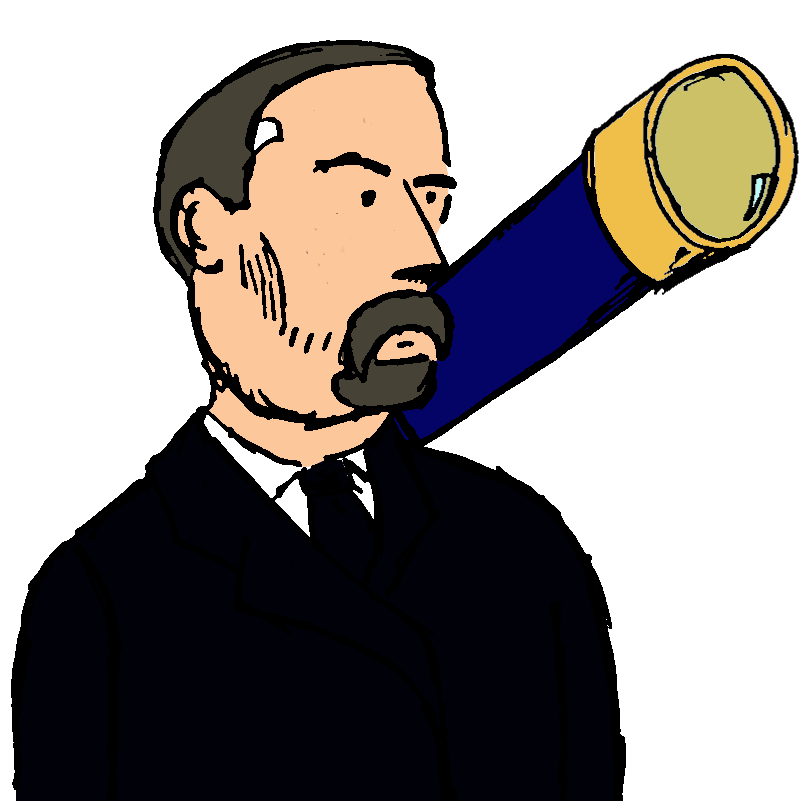
\includegraphics[width=12cm]{schiaparelli}};
		\end{scope}
		%
		\begin{scope}[shift={(0,-41)}]
			\draw [fill=space, ultra thick] (1,5) rectangle (29,-25);
			\draw [ultra thick, color=white] (6,0) circle (3cm);
			\foreach \i in {0,1,...,11}
				\draw [color=white, thick, rotate around={30*\i:(6,0)}] (6,2.8) -- (6,2.7);
			\draw [fill=white] (6,0) circle (0.1cm);
			\draw [thick, color=white] (6,0) -- (6,2.6);
			\draw [thick, color=white, rotate around={60:(6,0)}] (6,0) -- (6,1.5);
			%
			\node (example-textwidth-2) [right, align=left, text width=16cm, color=white, font=\fontsize{23pt}{24pt}\selectfont] at (11,0) {Il momento migliore per osservare le "stelle cadenti" è tra le 10 e le 4. Bisogna cercare un'ampia porzione di cielo in una zona scarsamente illuminata: ricordate che per abituare gli occhi al buio occorrono all'incirca 30 minuti.};
			%
			\begin{scope}[shift={(0,-7)}]
				\foreach \i in {1,2,...,10}{
					\pgfmathsetmacro{\x}{-10*rand}
					\pgfmathsetmacro{\y}{2*rand}
					\pgfmathsetmacro{\a}{45*rand}
					\pgfmathsetmacro{\opacVal}{rand*0.5+1}
					\begin{scope}[shift={(\x,-\y)}]
					\draw [rotate around={45:(14.8,-0.8)}, fill=white] (15,-1) to[out=180,in=270] (14.8,-0.8) to[out=90,in=180] (15,-0.6) -- (18,-0.6) -- (16,-0.8) -- (18,-1) -- (15,-1);
					\end{scope}
				}
			\end{scope}
			\node (example-textwidth-2) [right, align=left, text width=27cm, color=white, font=\fontsize{23pt}{24pt}\selectfont] at (1.5,-12.5) {Cadono all'incirca un centinaio di meteore all'ora, ma nel corso delle serate estive del 2020 si raggiungerà un massimo di circa 150 meteore all'ora, poiché quest'anno i percorsi di cometa e Terra sono particolarmente vicini.};
			%
			\begin{scope}
				\clip (3,-15) rectangle (28.5,-24);
				\draw [thick, color=black, fill=mars] plot [smooth cycle] coordinates {(2,-16) (5,-16) (10,-21) (5,-23) (2,-23)};
			\end{scope}
			\begin{scope}[scale=0.5,shift={(6,-18)}]
				\draw [thick, color=black, fill=earth] plot [smooth cycle] coordinates {(2,-16) (5,-16) (10,-21) (5,-23) (2,-23)};
			\end{scope}
			\draw [fill=dida,thick] (10.5,-15.8) rectangle (28.5,-22.5);
			\node (example-textwidth-2) [right, align=left, text width=17cm, color=black, font=\fontsize{23pt}{24pt}\selectfont] at (11,-19) {La velocità con cui entrano nell'atmosfera terrestre è di circa 216000 km/h. A questa velocità si riuscirebbe a coprire la distanza New York-Roma in poco meno di 2 minuti, o a compiere il giro dell'equatore terrestre in circa 11 minuti.};
		\end{scope}
		%
		\begin{scope}[shift={(0,-67)}]
			\node at (27,0) () {
\includegraphics[width=3.7cm]{licenza}};
			\node at (17.6,0.3) {\textcolor{black}{\fontsize{14}{15}\selectfont Fonte del testo: perseids su en.wiki e www.astroshop.eu}};
			\node at (18,-0.4) {\textcolor{black}{\fontsize{14}{15}\selectfont Grafica e illustrazioni: @ulaulaman - Gianluigi Filippelli}};
		\end{scope}
	\end{tikzpicture}
\end{document}